\subsection{CPU Architecture}
\label{subsec:interconnect-sc-background-cpu-arch}

Modern CPUs consist of many components, such as execution units, caches, PCIe root complex, and DRAM controllers.
Some subset of these components is always traversed when data is sent to or from the CPU to the PCIe endpoints.
The behaviour of each individual component may impact how the side-channel attack is carried out.
As such, it becomes necessary to understand all the components that may be involved in a PCIe transaction.

\begin{figure}[!htb]
    \centering
    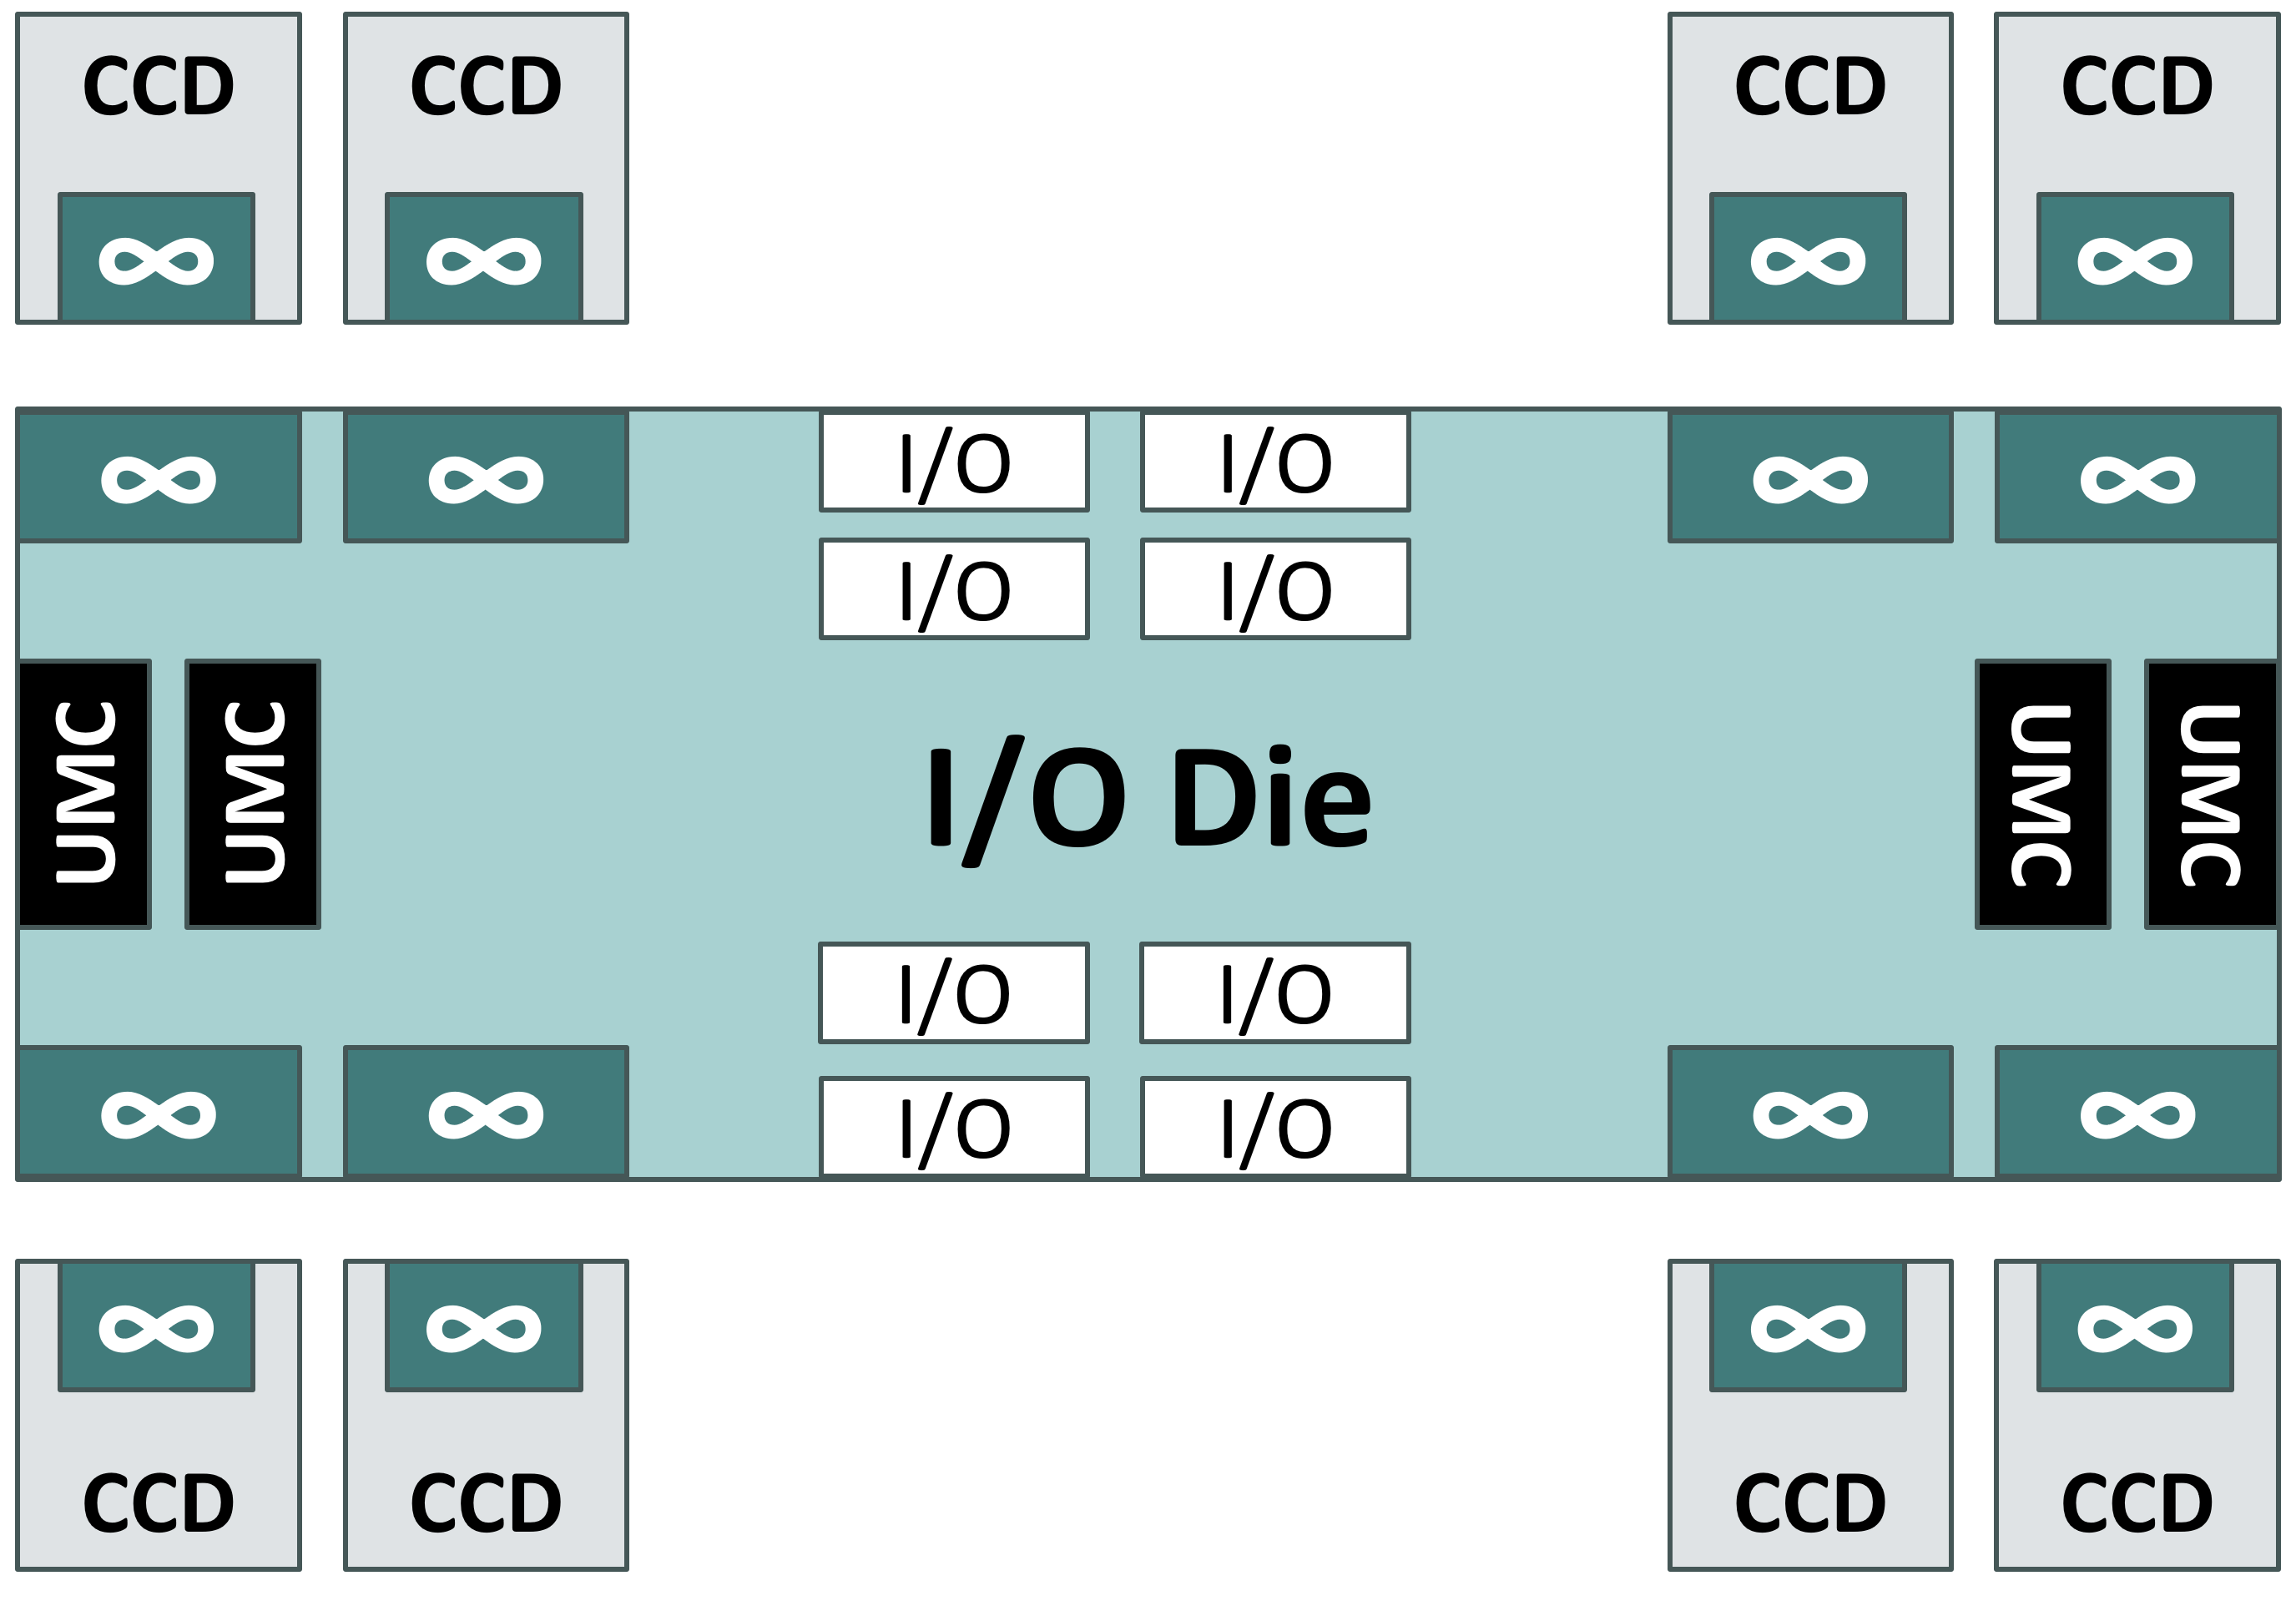
\includegraphics[width=\columnwidth]{figures/interconnect-sc/amd_arch/processor.png}
    \caption{AMD EPYC Zen 3 Architecture - CPU}
    \label{fig:amd-cpu}
\end{figure}


\Cref{fig:amd-cpu} shows a high-level overview of the architecture of the AMD EPYC Zen 3 processors.
The figure shows the following components:
\textbf{1) I/O:} The component that handles the input-output from the peripheral devices. This is where the PCIe communication happens.
\textbf{2) UMC:} The Unified Memory Controller is the controller that communicates with the DRAM.
\textbf{3) CCD:} The Core Complex Dies are where the cores (execution units) and caches reside.
\textbf{4) Infinity Fabric ($\infty$):} The interconnect that connects all of the components within the AMD CPU.

\subsubsection{CPU Pipelines}
\label{subsubsec:interconnect-sc-background-cpu-arch-pipelines}

Modern CPUs rely on executing multiple instructions simultaneously to maximise performance.
To achieve this, the CPUs have a multi-stage pipeline with the following stages: 1) Fetch, 2) Decode, 3) Schedule and Execute, and 4) Retire.
We provide a simplified view of the pipeline in the CPU cores of the AMD EPYC Zen 3 processors in \Cref{fig:amd-core} and a brief description of each of the stages below:\\
\textbf{Fetch: } This stage fetches the next macro-op from the cache or the memory. 
However, the next macro-op to be fetched may not be deterministic, given the program may contain branches. 
In such cases, this stage also uses branch prediction to speculate on which instruction may be executed next and fetch that instruction.\\
\textbf{Decode: } This stage involved decoding the fetched macro-op into one or more micro-ops, which are then forwarded to the next stages.\\
\textbf{Schedule and Execute: } The scheduler(s) determine which instruction can be executed next based on the availability of the data that the instruction requires. 
This ensures that a long-running instruction (e.g., where the data is unavailable) does not stall all other independent instructions that can be executed.
As such, instructions here can be executed out of program order. 
Once the instruction has finished execution and the output of the instruction (if any) is available in the registers, the instruction is removed from the scheduler.
As load and store are common but time-consuming instructions, this stage also consists of a load-store queue where pending load and store operations are held. \\
% \footnote{In Zen 3 cores, the load/store unit has a capacity of 72 loads and 64 stores.}. \\
\textbf{Retire: } This stage ensures that instructions are retired in the program order so that the program can remain oblivious to the out-of-order execution that occurred in the previous stage.

\begin{figure}[!htb]
    \centering
    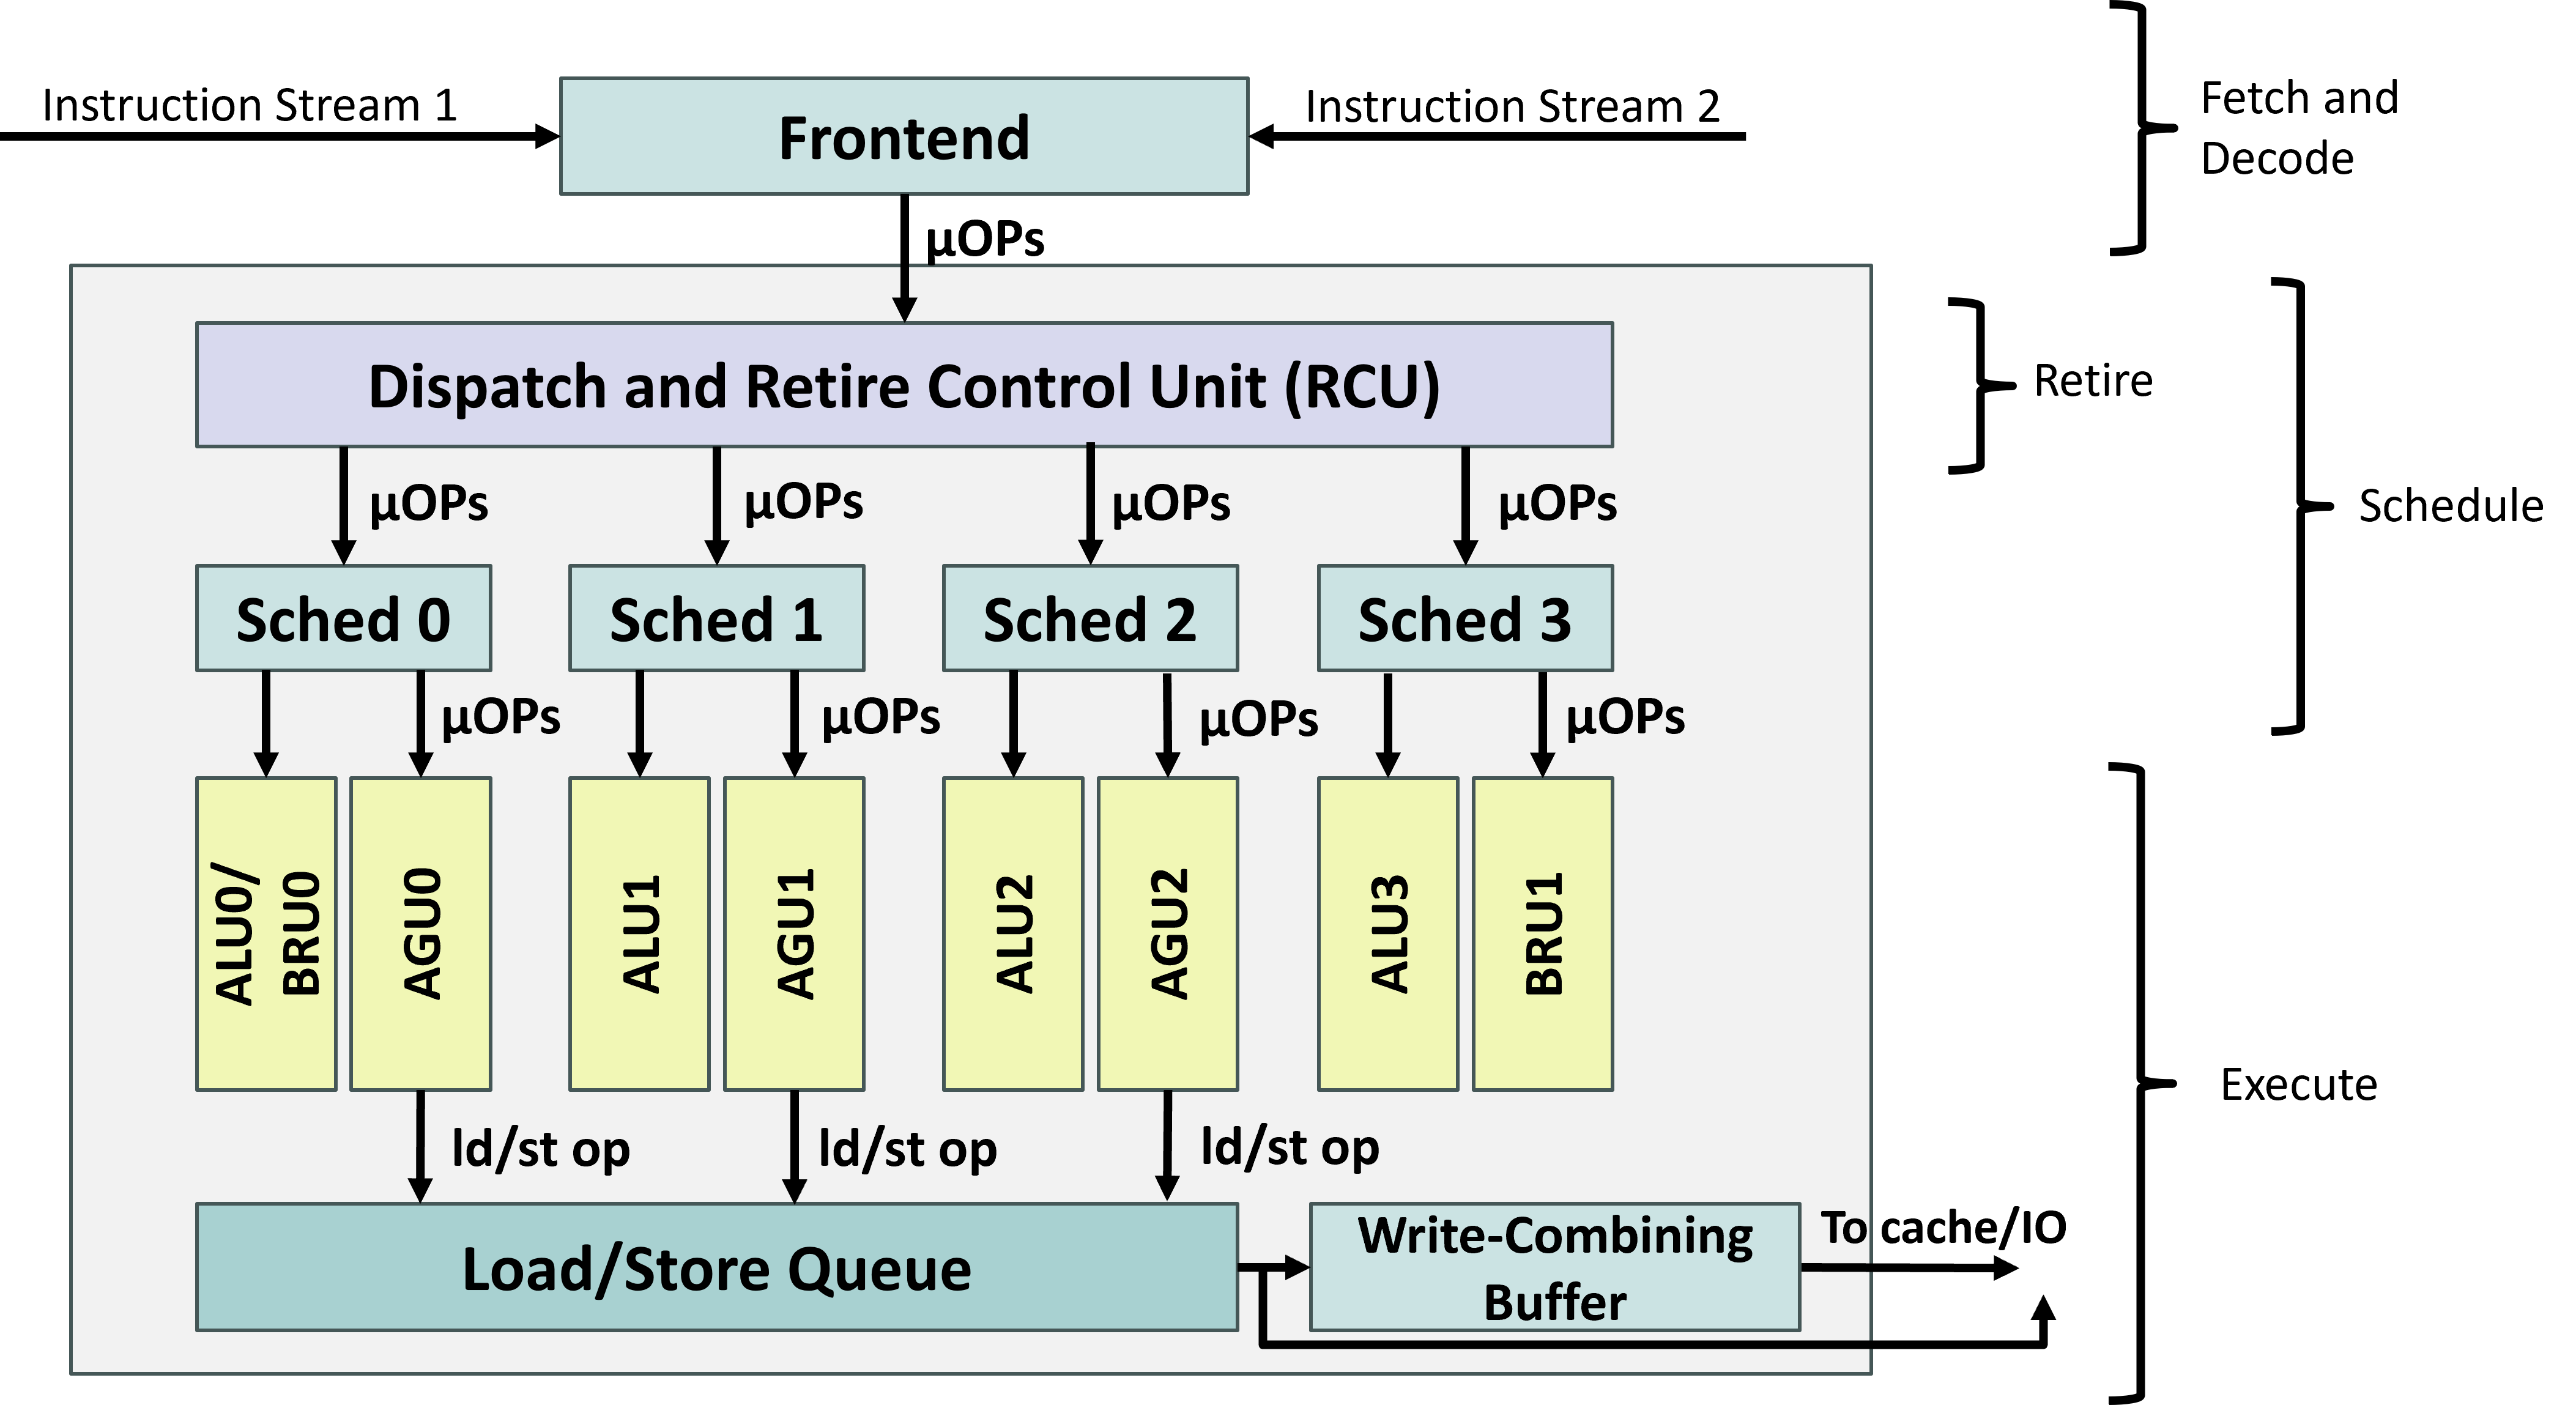
\includegraphics[width=\columnwidth]{figures/interconnect-sc/amd_arch/core.png}
    \caption{AMD EPYC Zen 3 Architecture - Core}
    \label{fig:amd-core}
\end{figure}

\subsubsection{PCIe transactions to/from CPU}
\label{subsubsec:interconnect-sc-background-cpu-arch-pcie-transactions}

A program running on the CPU can transfer data to the PCIe device/endpoint in two major ways: 1) Memory operations via memory-mapped IO (MMIO) and 2) Direct memory access (DMA).
MMIO enables the CPU to map some memory region of the PCIe endpoint in the CPU's physical address space.
Any process with the proper permissions can then map this memory within the process and perform normal \textit{load} or \textit{store} operations on this memory.
However, this approach requires the execution units of the CPU to issue repeated \textit{load/store} instructions to copy data to the PCIe endpoint.
While this method is useful for reading or writing limited content, such as small configuration parameters, to the PCIe endpoints, it is inefficient for transferring a large amount of data.
To alleviate this, many PCIe endpoints consist of a special hardware component called a direct memory access (DMA) engine.
The DMA engine is purpose-built to copy large chunks of contiguous data without involving the execution units of the CPU.

For MMIO-based transactions, the load or store instructions go through the same instruction pipeline outlined in \Cref{fig:amd-core}. 
From the Load Store Queue, they enter the I/O die shown in \Cref{fig:amd-cpu} and exit through the I/O block to the connected PCIe endpoint.
For DMA transactions, which are typically initiated by the PCIe endpoint, the transaction enters the I/O block. 
After address and protocol translations, they are transmitted to the DRAM through the UMC.